\documentclass[12pt]{article}
\usepackage{amsfonts} 
\usepackage{graphicx}
\usepackage{paralist}
\usepackage{hyperref}
\usepackage{xspace}
\usepackage{amsfonts}
\usepackage{amsmath}
\usepackage{graphicx}
\newcommand{\latex}{\LaTeX\xspace}
\oddsidemargin 0mm
\evensidemargin 0mm
\textwidth 160mm
\textheight 200mm
\renewcommand\baselinestretch{1.0}
\pagestyle {plain}
\pagenumbering{arabic}
\newcounter{stepnum}
\title{Assignment 4 Model \& View Specification}
\author{Yousam Asham, ashamy1}
\date{\today}
\begin {document}

\maketitle

\section*{Overview of Design}

This specification outlines how to construct the model and view modules of an MVC design pattern for a game of Dots. It consists of six modules in total.

The PointT module is an ADT to express certain points in a 2D sequence. This module is an integral part of this design since it make referencing certain points of the game board easier. It also minimizes the number of parameters passed into a lot of functions.

The ColourT module is a module that enumerates the five colours used in a Dots game. It also has a \verb|toString| method that maps each of the ColourT objects to their respective strings for ease of access in the PrintBoard module.

The RandomElem module is an interface module that provides a method called \verb|setRandElem|. This interface allows the developer to change the way that the digital board game generates its new elements, given a PointT object which indicates which entry in the board is should change.

The GameBoard module is a generic module that outlines the usage and modification of an abstract object through the usage of exported access programs. This abstract object is the GameBoard to be used. This module implements the RandomElem interface, however, since the GameBoard module is generic (meaning that the elements are not specified), the implemented \verb|setRandElem| method only sets the entry indicated by the PointT object to null since the GameBoard module is a generic module.

The DotsBoardT module is the main module for the model part of the MVC design pattern. It is essentially a GameBoard module but instead of being generic, it uses ColourT to satisfy the requirement of creating a model for a game of Dots.

The PrintBoard module is responsible for the view module which is part of the MVC design pattern.

This design considers many changes such as the following:

\begin{itemize}

\item The change to decide to create a different game that is similar to Dots in a sense that it uses a game board. The GameBoard module that is designed within this specification can be used to create a different digital board game that essentially requires the generation of new game elements after some have been removed.

\item It also allows for a change in the scoring system, as well as the level selection; this design allows for the changing of parameters to create new levels and add more challenging layers to a digital game.

\item In addition, the way that the elements on the game board can be referenced is also account for as part of change to this specification. The following specification uses a simple PointT module that can be used to construct PointT objects to reference specific points in the game board object. If a developer wishes to change this requirement, they are free to introduce a new way to referrence the game board elements instead of PointT objects.

\item Also, if a developer wishes to change their game's way of coming up with new elements for their game, they are free to do so through implementing the \verb|RandomElem| interface their own way.

\item Finally, if a developer wishes to change the actual objects that are the elements of the game board (i.e. the ColourT objects in this specification), they are free to do so by just changing the ColourT to suit their element type of choice.

\end{itemize}

\newpage

\section* {Point ADT Module}

\subsection*{Template Module}

PointT

\subsection* {Uses}

N/A

\subsection* {Syntax}

\subsubsection* {Exported Types}

PointT = ?

\subsubsection* {Exported Access Programs}

\begin{tabular}{| l | l | l | l |}
\hline
\textbf{Routine name} & \textbf{In} & \textbf{Out} & \textbf{Exceptions}\\
\hline
PointT & $\mathbb{Z}$, $\mathbb{Z}$ & PointT & \\
\hline
row & ~ & $\mathbb{Z}$ & ~\\
\hline
col & ~ & $\mathbb{Z}$ & ~\\
\hline
\end{tabular}

\subsection* {Semantics}

\subsubsection* {State Variables}

$r$: $\mathbb{Z}$\\
$c$: $\mathbb{Z}$

\subsubsection* {State Invariant}

None

\subsubsection* {Assumptions}

The constructor PointT is called for each object instance before any other
access routine is called for that object.  The constructor cannot be called on
an existing object.

\subsubsection* {Access Routine Semantics}

PointT($row, col$):
\begin{itemize}
\item transition: $r, c := row, col$
\item output: $out := \mathit{self}$
\item exception: None
\end{itemize}

\noindent row():
\begin{itemize}
\item output: $out := r$
\item exception: None
\end{itemize}

\noindent col():
\begin{itemize}
\item output: $out := c$
\item exception: None
\end{itemize}

\newpage


\section* {ColourT Module}

\subsection*{Module}

ColourT

\subsection* {Uses}

None

\subsection* {Syntax}

\subsubsection* {Exported Constants}

None

\subsubsection* {Exported Types}

ColourT = \{blue, green, purple, orange, red\} //$Enumerated$

\subsubsection* {Exported Access Programs}

\begin{tabular}{| l | l | l | p{5.5cm} |}
\hline
\textbf{Routine name} & \textbf{In} & \textbf{Out} & \textbf{Exceptions}\\
\hline
toString &  &  & \\
\hline

\end{tabular}

\subsection*{Semantics}

\subsubsection*{State Variables}

None

\subsubsection*{State Invariant}

None

\subsubsection*{Assumptions}

None

\subsection*{Access Routine Sematics}

\noindent toString():

\begin{itemize}

\item output: $out:= self = \mbox{blue} \Rightarrow \mbox{"Blue"} \mid  self = \mbox{green} \Rightarrow \mbox{"Green"} \mid  self = \mbox{purple} \Rightarrow \mbox{"Purple"} \mid self = \mbox{orange} \Rightarrow \mbox{"Orange"} \mid \mbox{true} \Rightarrow \mbox{"Red"}$

\item exception: none.

\end{itemize}

\newpage

\section* {RandomElem Interface Module}

\subsection*{Generic Module}

RandomElem

\subsection* {Uses}

PointT

\subsection* {Syntax}

\subsubsection* {Exported Constants}

None

\subsubsection* {Exported Types}

None
\subsubsection* {Exported Access Programs}

\begin{tabular}{| l | l | l | p{5.5cm} |}
\hline
\textbf{Routine name} & \textbf{In} & \textbf{Out} & \textbf{Exceptions}\\
\hline
setRandElem & PointT &  &IndexOutOfBoundsException\\
\hline
\end{tabular}

\newpage

\section* {Generic GameBoard Module inherits RandomElem interface}

\subsection*{Generic Module}

GameBoard(T)

\subsection* {Uses}

PointT, RandomElem

\subsection* {Syntax}

\subsubsection* {Exported Constants}

SIZE = 6 //$size$ $of$ $the$ $board$ $in$ $each$ $direction$ 

\subsubsection* {Exported Types}

None
\subsubsection* {Exported Access Programs}

\begin{tabular}{| l | l | l | p{5.5cm} |}
\hline
\textbf{Routine name} & \textbf{In} & \textbf{Out} & \textbf{Exceptions}\\
\hline
init & seq of (seq of T), $\mathbb{N}, \mathbb{N}$, T &  &\\
\hline
getBoard & & seq of (seq of T) & \\
\hline
getElement & PointT &  & IndexOutOfBoundsException \\
\hline
getScore & & $\mathbb{N}$ & \\
\hline
getMoves & & $\mathbb{N}$ & \\
\hline
getTargetMoves & & $\mathbb{N}$ & \\
\hline
getTargetScore & & $\mathbb{N}$ & \\
\hline
getTargetType & & T & \\
\hline
popElems & seq of PointT &  &IndexOutOfBoundsException, IllegalArgumentException, ArithmeticException\\
\hline
remove & PointT & & IndexOutOfBoundsException \\
\hline
rebase & & & \\
\hline
setRandElem&PointT& & IndexOutOfBoundsException\\
\hline
has\_won & & $\mathbb{B}$ & \\
\hline

\end{tabular}

\subsection* {Semantics}

\subsubsection* {State Variables}

$g$: seq of (seq of T)\\
$score$: $\mathbb{N}$\\
$moves$: $\mathbb{N}$\\
$targetMoves$: $\mathbb{N}$\\
$targetScore$: $\mathbb{N}$\\
$targetElement$: T\\

\subsubsection* {State Invariant}

count(T\textsubscript{0}) + count(T\textsubscript{1}) + count(T\textsubscript{2}) + ... + count(T\textsubscript{n}) = SIZE*SIZE

\noindent//$Where\, n\, represents\, the\, quantity\, of\, the\, number\, of\, elements\, in\, the\, type\, \mbox{T}$

\subsubsection* {Assumptions}

\begin{itemize}

\item The init method is called for the abstract object before any other access routine is called for that object. The init method can be used to return the state of the game to the state of a new game.

\item There exists a function called random() that returns a number between 0 and 1.
\end{itemize}
\subsubsection*{Access Routine Semantics}

init(s, tm, ts, te):

\begin{itemize}

\item transition: $g, score, moves, targetMoves, targetScore, targetElement := s, 0, 0, tm, ts, te$

\item exception: none.

\end{itemize}

\noindent getElement($p$):

\begin{itemize}

\item output: $out := g[p.row][p.col]$

\item exception: $exc := \lnot (\mbox{validPoint}(p)) \Rightarrow$ IndexOutOfBoundsException

\end{itemize}

\noindent getBoard():

\begin{itemize}

\item output: $out := g$

\item exception: none.

\end{itemize}

\noindent getScore():

\begin{itemize}

\item output: $out := score$

\item exception: none.

\end{itemize}

\noindent getMoves():

\begin{itemize}

\item output: $out := moves$

\item exception: none.

\end{itemize}

\noindent getTargetMoves():

\begin{itemize}

\item output: $out := targetMoves$

\item exception: none.

\end{itemize}

\noindent getTargetScore():

\begin{itemize}

\item output: $out := targetScore$

\item exception: none.

\end{itemize}

\noindent getTargetType():

\begin{itemize}

\item output: $out := targetelement$

\item exception: none.

\end{itemize}

\noindent popElems($s$):

\begin{itemize}

\item transition: $score, moves := score + +(p:\mbox{PointT}\mid p \in s \land g[p.row][p.col] = targetColour:1), moves+1$
\item exception: exc := $\exists (p : $PointT$\mid p \in s$ $: \lnot$validPoint($p$)$) \Rightarrow$ IndexOutOfBoundsException $\mid \lnot$(isAdjList$(s)) \lor (|s| < 2) \lor \lnot(\mbox{sameColour}(s))\Rightarrow$ IllegalArgumentException $\mid moves > targetMoves \Rightarrow$ ArithmeticException

\end{itemize}

\noindent remove($p$):

\begin{itemize}

\item transition: $g[p.row][p.col]= null$

\item exception: $exc:=\lnot (\mbox{validPoint}(p)) \Rightarrow$ IndexOutOfBoundsException

\end{itemize}

\noindent rebase():

\begin{itemize}

\item transition: $g[i][j] = null \land \lnot(\mbox{validRowCol}(i-1)) \Rightarrow g[i][j] := \mbox{getRandElem}((10*random())\%5) \mid g[i][j] = null \land g[i-1][j] \ne null \Rightarrow g[i][j], g[i-1][j] := g[i][j-1], null$. This happens repeatedly while iterating through all the rows of the game board (excluding the first row, $i=0$), SIZE times. The end state of the game board should satisfy $\forall (p: \mbox{PointT}\mid \mbox{validPoint}(p):g[p.row][p.col] \ne null)$ This is to re-populate the game board.

\item exception: none.

\end{itemize}

\noindent setRandElem($p$):

\begin{itemize}

\item transition: $g[p.row][p.col] = null$

\item exception: $exc:= \lnot (\mbox{validPoint}(p)) \Rightarrow$ IndexOutOfBoundsException

\end{itemize}

\noindent has\_won():

\begin{itemize}

\item output: $out:= (moves \le targetMoves) \land (score \ge targetScore)$

\item exception: none.

\end{itemize}

\newpage

\subsection*{Local Functions}

\noindent isAdjList: seq of PointT $\rightarrow \mathbb{B}$\\
isAdjList($s$) $\equiv \forall(i:\mathbb{N} \mid 0 \le i \le \lvert s\rvert - 2$ : $(s[i].row = s[i+1].row-1) \lor (s[i].row=s[i+1].row+1) \lor (s[i].col=s.col[i+1]-1) \lor (s[i].col=s[i+1].col+1) \land \lnot((s[i].row = s[i+1].row +1)\land (s[i].col = s[i+1].col+1))\land \lnot ((s[i].row = s[i+1].row-1)\land (s[i].col = s[i+1].col-1))$\\

\noindent validRowCol:$\mathbb{N} \rightarrow \mathbb{B}$\\
validPoint($i$)$ \equiv (0 \le i < SIZE)$\\

\noindent validPoint: PointT $\rightarrow \mathbb{B}$\\
validPoint($p$)$ \equiv $ validRowCol($p.row$) $\land$ validRowCol($p.col$) \\

\noindent sameColour: seq of PointT $\rightarrow \mathbb{B}$\\
sameColour($s$) $\equiv \forall(i:\mathbb{N} \mid 0 \le i \le \lvert s \rvert -2 : g[s[i].row][s[i].col]= g[s[i+1].row][s[i+1].col])$\\

\newpage

\section* {DotsBoardT Module and inherits the RandomElem interface}

\subsection*{Module}

DotsBoardT is GameBoard(ColourT)

\subsection* {Uses}

PointT, RandomElem, GameBoard

\subsection* {Syntax}

\subsubsection* {Exported Constants}

SIZE = 6 //$size$ $of$ $the$ $board$ $in$ $each$ $direction$ 

\subsubsection* {Exported Types}

None
\subsubsection* {Exported Access Programs}

\begin{tabular}{| l | l | l | p{5.5cm} |}
\hline
\textbf{Routine name} & \textbf{In} & \textbf{Out} & \textbf{Exceptions}\\
\hline
setRandElem& PointT & & IndexOutOfBoundsException\\
\hline
\end{tabular}

\subsection* {Semantics}

\subsubsection* {State Invariant}

count(blue) + count(green) + count(purple) + count(orange) + count(red) = SIZE*SIZE

\subsubsection* {Assumptions}

\begin{itemize}

\item The init method is called for the abstract object before any other access routine is called for that object. The init method can be used to return the state of the game to the state of a new game.

\item There exists a function called random() that returns a number between 0 and 1.
\end{itemize}
\subsubsection*{Access Routine Semantics}

\noindent setRandElem($p$):

\begin{itemize}

\item transition: $g[p.row][p.col] = \mbox{getRandomElem()}$

\item exception: $exc:= \lnot \mbox{validPoint}(p) \Rightarrow$ IndexOutOfBoundsException.

\end{itemize}

\newpage

\subsection*{Local Functions}

\noindent getRandomElem: ColourT\\
getRandomElem() $\equiv 0 < \mbox{random()} \le 0.2  \Rightarrow blue \mid 0.2 < \mbox{random()} \le 0.4 \Rightarrow green \mid 0.4 < \mbox{random()} \le 0.6 \Rightarrow purple \mid 0.6 < \mbox{random()} \le 0.8 \Rightarrow orange \mid 0.8 < \mbox{random()} \le 1.0 \Rightarrow red$\\

\noindent isAdjList: seq of PointT $\rightarrow \mathbb{B}$\\
isAdjList($s$) $\equiv \forall(i:\mathbb{N} \mid 0 \le i \le \lvert s\rvert - 2$ : $(s[i].row = s[i+1].row-1) \lor (s[i].row=s[i+1].row+1) \lor (s[i].col=s.col[i+1]-1) \lor (s[i].col=s[i+1].col+1) \land \lnot((s[i].row = s[i+1].row +1)\land (s[i].col = s[i+1].col+1))\land \lnot ((s[i].row = s[i+1].row-1)\land (s[i].col = s[i+1].col-1))$\\

\noindent validRowCol:$\mathbb{N} \rightarrow \mathbb{B}$\\
validPoint($i$)$ \equiv (0 \le i < SIZE)$\\

\noindent validPoint: PointT $\rightarrow \mathbb{B}$\\
validPoint($p$)$ \equiv $ validRowCol($p.row$) $\land$ validRowCol($p.col$) \\

\noindent sameColour: seq of PointT $\rightarrow \mathbb{B}$\\
sameColour($s$) $\equiv \forall(i:\mathbb{N} \mid 0 \le i \le \lvert s \rvert -2 : g[s[i].row][s[i].col]= g[s[i+1].row][s[i+1].col])$\\

\noindent count: T $\rightarrow \mathbb{N}$\\
count($e$) $\equiv +(p:$PointT$\mid \mbox{validPoint}(p) \land g[p.row][p.col] = e: 1)$\\

\newpage

\section* {PrintBoard Module}

\subsection*{Module}

PrintBoard

\subsection* {Uses}

ColourT, PointT, GameBoard

\subsection* {Syntax}

\subsubsection* {Exported Constants}

None

\subsubsection* {Exported Types}

PrintBoard = ?

\subsubsection* {Exported Access Programs}

\begin{tabular}{| l | l | l | p{5.5cm} |}
\hline
\textbf{Routine name} & \textbf{In} & \textbf{Out} & \textbf{Exceptions}\\
\hline
new PrintBoard& seq of (seq of ColourT) & Print & IllegalArgumentException\\
\hline
getElem & PointT & ColourT & IndexOutIOfBoundsException\\
\hline
print& & & \\
\hline

\end{tabular}

\subsection* {Semantics}

\subsubsection*{Environmental Variables}

$screen$: a two dimensional sequence of positions on the screen, where each position holds a character.

\subsubsection* {State Variables}
$g:$ seq of (seq of characters)

\subsubsection* {State Invariant}

None

\subsubsection* {Assumptions}

\begin{itemize}

\item The constructor is called for the class before any other access routine is called for that object.

\end{itemize}
\subsubsection*{Access Routine Semantics}

new PrintBoard(s):

\begin{itemize}

\item transition: $s[i][j] = \mbox{ColourT.blue} \Rightarrow g[i][j] := \mbox{'b'} \mid s[i][j] = \mbox{ColourT.green} \Rightarrow g[i][j] := \mbox{'g'} \mid s[i][j] = \mbox{ColourT.purple} \Rightarrow g[i][j] := \mbox{'p'} \mid s[i][j] = \mbox{ColourT.orangle} \Rightarrow g[i][j] := \mbox{'o'} \mid s[i][j] = \mbox{ColourT.red} \Rightarrow g[i][j] := \mbox{'r'}$ such that $i:\mathbb{N}$, $j:\mathbb{N}$ iterate over the every element in s.

\item output: $out := self$

\item exception: $exc := $ An element in s is not of type ColourT $\Rightarrow$ IllegalArgumentException.

\end{itemize}

\noindent getElem($p$):

\begin{itemize}

\item output: $out := g[p.row][p.col]$

\item exception: $exc := \lnot (\mbox{validPoint}(p)) \Rightarrow$ IndexOutOfBoundsException.

\end{itemize}

\noindent print():

\begin{itemize}

\item transition: Change the state of $screen$ by changing the element returned by getElem$(p)$, where the state variables of $p$: PointT are changed so every element of the board is returned sequentially row by row with a newline charachter being printed every DotsBoard.SIZE elements, changing the state of $screen$ to be on the next row. After the last row, the $score$, $moves$, $targetMoves$, $targetScore$, and the $targetElement$ is displayed on $screen$ in the format "$score$/$targetScore$    $moves$/$targetMoves$	      Target: $targetElement$"

\item exception: none

\end{itemize}

\newpage
\subsection*{Local Functions}

\noindent validPoint: PointT $\rightarrow \mathbb{B}$\\
validPoint($p$)$ \equiv $ validRowCol($p.row$) $\land$ validRowCol($p.col$) \\

\noindent validRowCol:$\mathbb{N} \rightarrow \mathbb{B}$\\
validPoint($i$)$ \equiv (0 \le i < SIZE)$\\

\newpage

\section*{Specification Critique}

This specifcation was very challenging and thought provoking to come up with. I had to make a lot of design decisions in the process such as: whether the \verb|setRandElem| method should be included in the MIS as an interface or just an exported access program that is included within the ColourT module. I decided to include it in an interface; that way the selection of a new element entry can be customized based on the game to be implemented. This supports the design for change principle talked about earlier in the semester.

In terms of software qualities, this specification is pretty consistent. This is because formal language (discrete maths) was used to explain what each of the access programs (and local functions) did. However, there were some parts that were not understandable if discrete math formal language was used; for these parts some informal language had to be used. I have tried to make this specification as consistent as possible. Also, adding the PointT module to this specification made it more consistent since now all the points in a 2D sequence can be referenced using a standardized way, which is with the use of a PointT object.

This specification is mostly essential. Keeping this specification essential was hard since I had to separate the move of popping dots into three stages that had to be independent of each other. These three stagees are represented by the following three method of the GameBoard module: \verb|popElem, remove, rebase|.

As for generality, this specification would be high scoring. The GameBoard module is general since it is generic. Moreover, the choice to have the RandomElem interface adds more generality to this specification since it has gives the option for the usage of other randomization/non-randomization methods.

This specification had to sacrifice some minimality. This can be seen in the \verb|popElems()| method in the GameBoard module. This sacrifice had to be made since it would be too much work for a controller to call two separate methods one changing the score while the other changes the number of moves already taken in a dots game. This sacrifice had to be made for the sake of usability. I also had the option to combine the \verb|remove| and the \verb|rebase| methods into one method (since they both change only one state variable, the grid) but this would have made the resulting method a large one that would be hard to understand. Anyways, both of these options would be considered minimal.

In terms of cohesion, I believe that all of these modules go and work well together. The only module that would be hard to connect to the other would be the PrintBoard module, however, this module had to be included to serve as the main module for the view module of an MVC design pattern.

Information hiding was well maintained through out the implementation and the specification. To make sure of that, all the local functions were implemented as private functions, and the state variables were declared as \verb|protected|. Also, since the specification maintains generality, this means that it maintains design for change. Design for change is an influencing factor of information hiding.

\section*{Answers to questions}

\begin{enumerate}

\item Proxy pattern: The proxy pattern allows for an intermediary object between a client trying to communicate to a component. This intermediary object can be seen as a representative of the component that the client is trying to communicate to. This design pattern is usually used to prevent the client from accessing a component that is unsafe or non-secure. This design pattern would be used while browsing to help keep the client safe while browsing the web and to make sure that the wesites the client would be accessing are safe websites.

Adapter pattern: The adapter pattern is used to accomodate two incompatible interfaces. For example, in a video game, there is a HumanPerson interface that defines what a human can do as exported access programs such as \verb|walk()| and \verb|jump()|. However if you wanted to instantiate an object thats not human (suppose that object we need to instantiate is a basketball), the ball cannot perform the same actions as a human. Therefore the developer would need an adapter class that would implement methods \verb|walk()| that points to a different method called \verb|roll()|, and it would implement the \verb|jump()| method to point to a method called \verb|bounce()|. This is how an adapter design pattern could be used.

Strategy pattern: The strategy design pattern allows for the creation of an interface and then creating a class that implements that interface in two ways, and all of that would happen in one module. For example, suppose we have a Animal super class and a dog module that extends the Animal module and a bird module that also extends the Animal module. In order to give the dog and the bird flying abilities (or something to indicate if they can fly or not), we would create a FlyOrNo interface and within that interface module we could define two classes (one called CanFly while the other is called CantFly) that has access programs that implement that FlyOrNo interface so that it could fly, and the other class implements it as if they cannot fly. It would then add a new instance variable pertaining to whether the animal has the ability to fly or not. This type of design pattern would avoid repetition of code within the dog and the bird class and will instead make use of an instance variable to indicate whether an animal could fly or not.

All of these design patterns allow the developer to implement their code without any loss of generality and therefore lead to abstraction. All these design patterns allow for designing with change in mind. If any changes need to be made to the implementation of one of these design patterns the change would not be problematic and would be easy to make.

\item \noindent

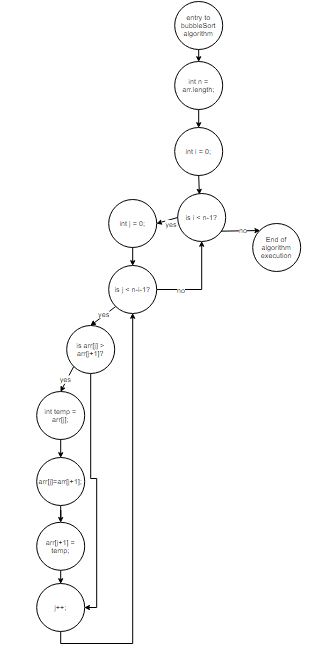
\includegraphics{cfg.png}

\end{enumerate}

\end {document}
